\chapter{绘制杯立体图}
{\bfseries 知识目标}
\begin{itemize}
\item 掌握line命令的使用
\item 掌握offset命令和trim命令的使用
\item 掌握AutoCAD视图切换知识
\item 掌握AutoCAD旋转和拉伸建模命令的使用方法
\end{itemize}

{\bfseries 技能目标}
\begin{itemize}
\item 能够根据给定的回转体零件图,运用投影知识选择正确的投影图
\item 能够根据块零件特征,运用AutoCAD命令,绘制特征图
\item 能够运用AutoCAD旋转和拉伸命令,完成回转体零件的三绘建模
\end{itemize}

{\bfseries 本章提要}

本章将对调压阀中的杯零件进行三维建模,使读者能够掌握line命令、offset命令和trim命令绘制简单回转体零件特征视图的方法,并通过实体建模中revolve命令和extude命令来生成三维模型。通过完成该项目读者能够基本掌握使用AutoCAD进行三维建模的基本步骤。图\ref{fig:tiaoyafabei}所示即为本项目的块零件图。
\noindent
\begin{figure}[htbp]
\centering
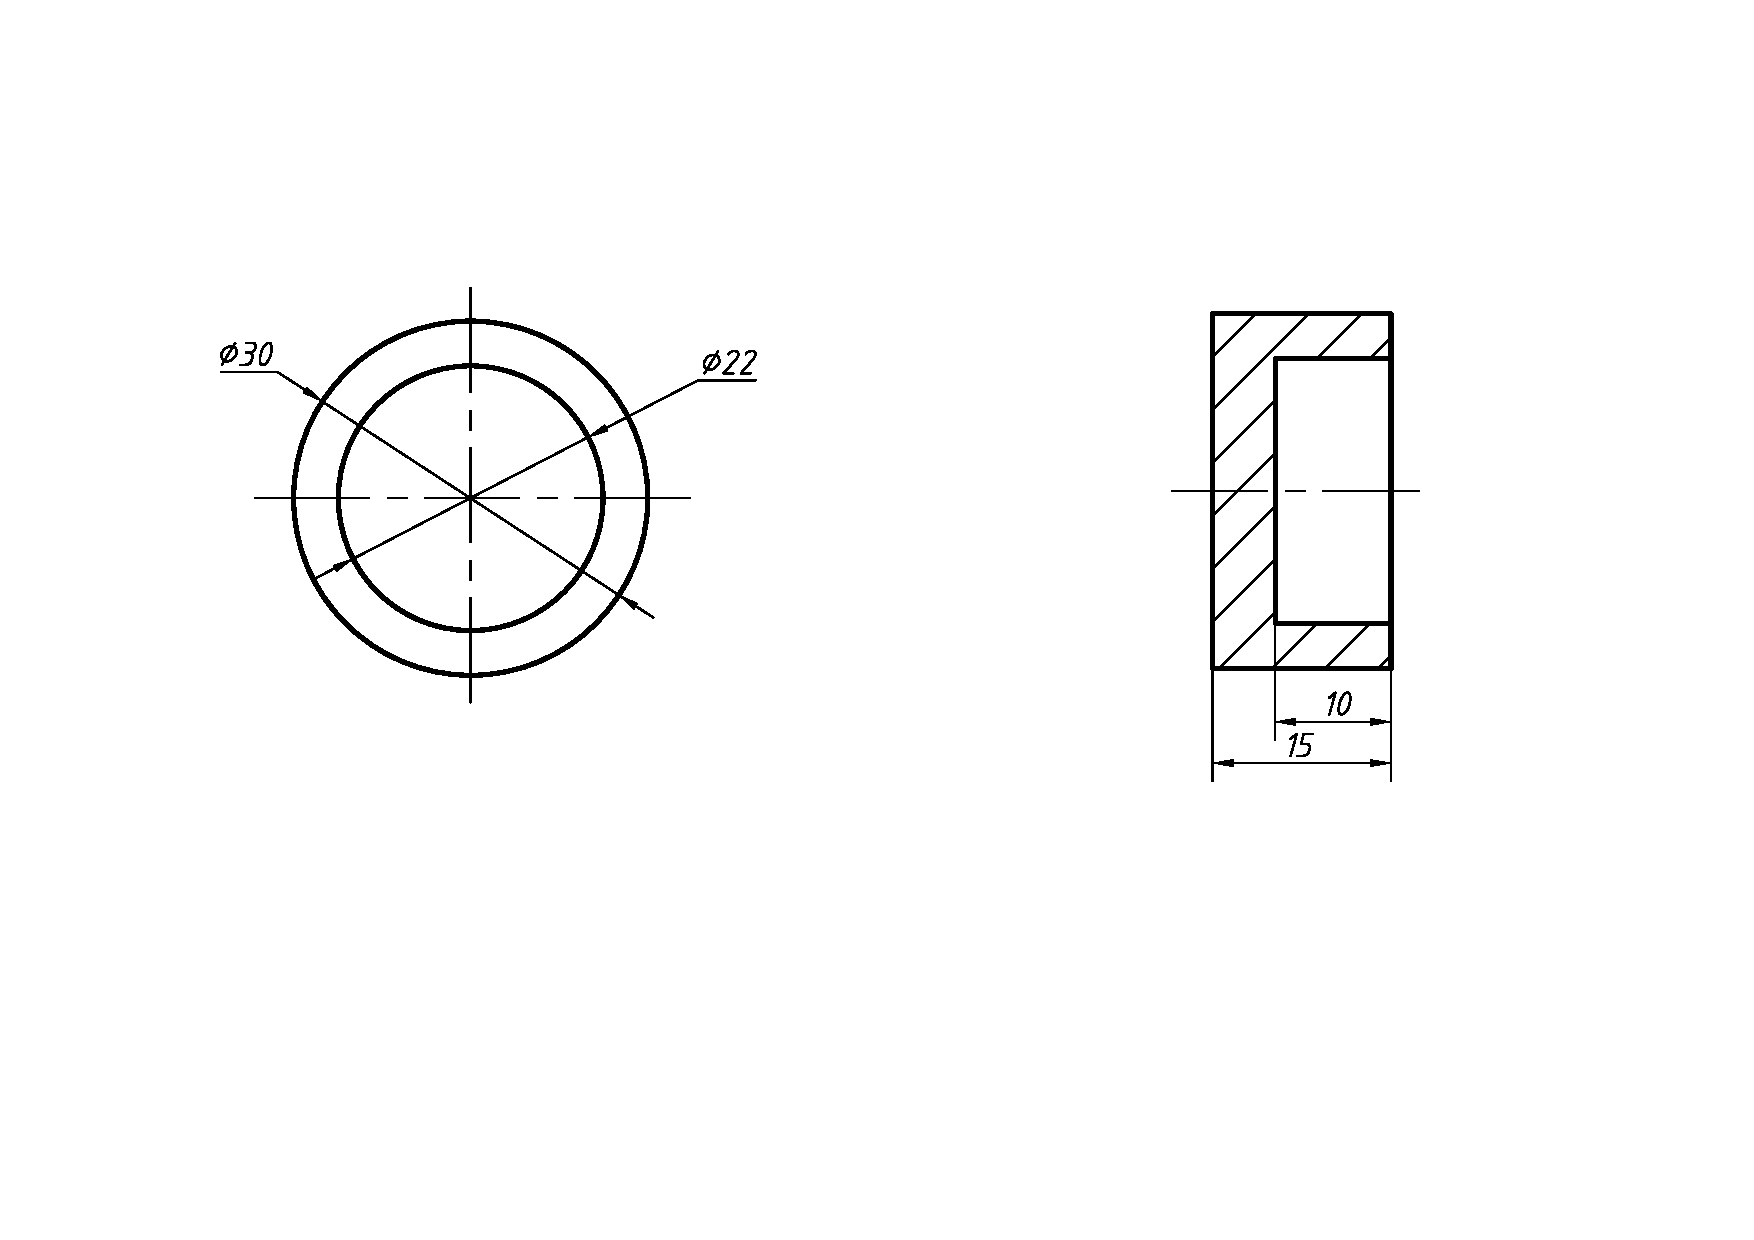
\includegraphics[scale=0.6]{tiaoyafabei.pdf}
\caption{调压阀杯块零件图}\label{fig:tiaoyafabei}
\end{figure}
\endinput